%	This is written by Zhiyang Ong as a template for writing reports.

%	The MIT License (MIT)

%	Copyright (c) <2014> <Zhiyang Ong>

%	Permission is hereby granted, free of charge, to any person obtaining a copy of this software and associated documentation files (the "Software"), to deal in the Software without restriction, including without limitation the rights to use, copy, modify, merge, publish, distribute, sublicense, and/or sell copies of the Software, and to permit persons to whom the Software is furnished to do so, subject to the following conditions:

%	The above copyright notice and this permission notice shall be included in all copies or substantial portions of the Software.

%	THE SOFTWARE IS PROVIDED "AS IS", WITHOUT WARRANTY OF ANY KIND, EXPRESS OR IMPLIED, INCLUDING BUT NOT LIMITED TO THE WARRANTIES OF MERCHANTABILITY, FITNESS FOR A PARTICULAR PURPOSE AND NONINFRINGEMENT. IN NO EVENT SHALL THE AUTHORS OR COPYRIGHT HOLDERS BE LIABLE FOR ANY CLAIM, DAMAGES OR OTHER LIABILITY, WHETHER IN AN ACTION OF CONTRACT, TORT OR OTHERWISE, ARISING FROM, OUT OF OR IN CONNECTION WITH THE SOFTWARE OR THE USE OR OTHER DEALINGS IN THE SOFTWARE.

%	Email address: echo "cukj -wb- 23wU4X5M589 TROJANS cqkH wiuz2y 0f Mw Stanford" | awk '{ sub("23wU4X5M589","F.d_c_b. ") sub("Stanford","d0mA1n"); print $5, $2, $8; for (i=1; i<=1; i++) print "6\b"; print $9, $7, $6 }' | sed y/kqcbuHwM62z/gnotrzadqmC/ | tr 'q' ' ' | tr -d [:cntrl:] | tr -d 'ir' | tr y "\n"

%%%%%%%%%%%%%%%%%%%%%%%%%%%%%%%%%%%%%%%%%%%%%%


%%%%%%%%%%%%%%%%%%%%%%%%%%%%%%%%%%%%%%%%%%%
\section{Conclusion}
\label{sec:Conclusion}

%By examining the different microarchitectural implementations of the {\it MIPS} ISA, we can conclude that the ISA determines various aspects of a microarchitecture for that ISA. For example, the microarchitecture for a RISC processor would have a simpler control unit/path than the microarchitecture for a CISC processor. Also, we can observe that the microarchitecture design of a processor affects the performance of the computer system, since the clock rate (CCT) and the CPI for the processor is determined by its microarchitecture \cite{Patterson2005}. \\
By examining the different microarchitectural implementations of the {\it MIPS} ISA, we can conclude that the ISA determines various aspects of a microarchitecture for that ISA. For example, the microarchitecture for a multi-cycle processor (see Figure \ref{fig:multicycleprocessor}) would have a simpler control unit/path than the microarchitecture for a pipelined processor (see Figure \ref{fig:pipelinedprocessor}). Also, we can observe that the microarchitecture design of a processor affects the performance of the computer system, since the clock rate (CCT) and the CPI for the processor is determined by its microarchitecture \cite{Patterson2005}. \\

Furthermore, there is a trade-off between hardware complexity (and hence, design effort and power consumption) and performance for the three scalar processor architectures (single-cycle, multi-cycle, and pipelined processors) that are considered. Microarchitectures that have better performance have more hardware complexity, in terms of the datapath and the control path. For example, the aforementioned multi-cycle processor performs better than the single-cycle processor at the cost of more hardware complexity (in the datapath and the control path). Also, the pipelined processor trades off more hardware complexity than the multi-cycle processor for better performance. However, as we add move to superscalar and superpipelined microarchitectures \cite{Jouppi1989}, we have to consider a more nuanced trade-off between hardware complexity for the issue logic, instructions per cycle (IPC) (see Equation \ref{eqn:ipcandcpi} for its definition), and computer performance \cite{Hrishikesh2002,Palacharla1998}. Comparing a heavily pipelined processor architecture to a not-so-heavily pipelined processor, the former may have worse performance than the latter, since the former would have a greater proportion of pipeline overhead per clock cycle. It means that the heavily pipelined processor wastes more computational resources for inefficient work than the not-so-heavily pipelined processor. Similarly, when comparing a superscalar processor with a wider instruction issue width to another superscalar processor of narrower instruction issue width, the former would have greater inefficiency than the latter. This is because the former would have greater hardware complexity (in terms of logic/circuit and wiring complexities) than the latter. Also, after issuing instructions in order, the former would spend more computational resources than the latter in trying to execute instructions out of order and retiring them in order \cite{Shen2005a,Hennessy2012}. \\
%An heavily pipelined processor architecture may have worse performance than a less pipelined processor, since the heavily pipelined processor architecture would have a greater proportion of pipeline overhead per clock cycle for inefficient work in comparison to the less pipelined processor. 
%Similarly, the hardware complexity (in terms of logic/circuit and wiring complexities) for a superscalar processor that has a wider instruction issue width would have greater inefficiency than superscalar processors of narrower instruction issue width in spending computational resources trying to execute instructions out of order and 

%	Figure 6.52 and 6.53, Patterson2005, pp. 453

\begin{figure}[h]
\centering 
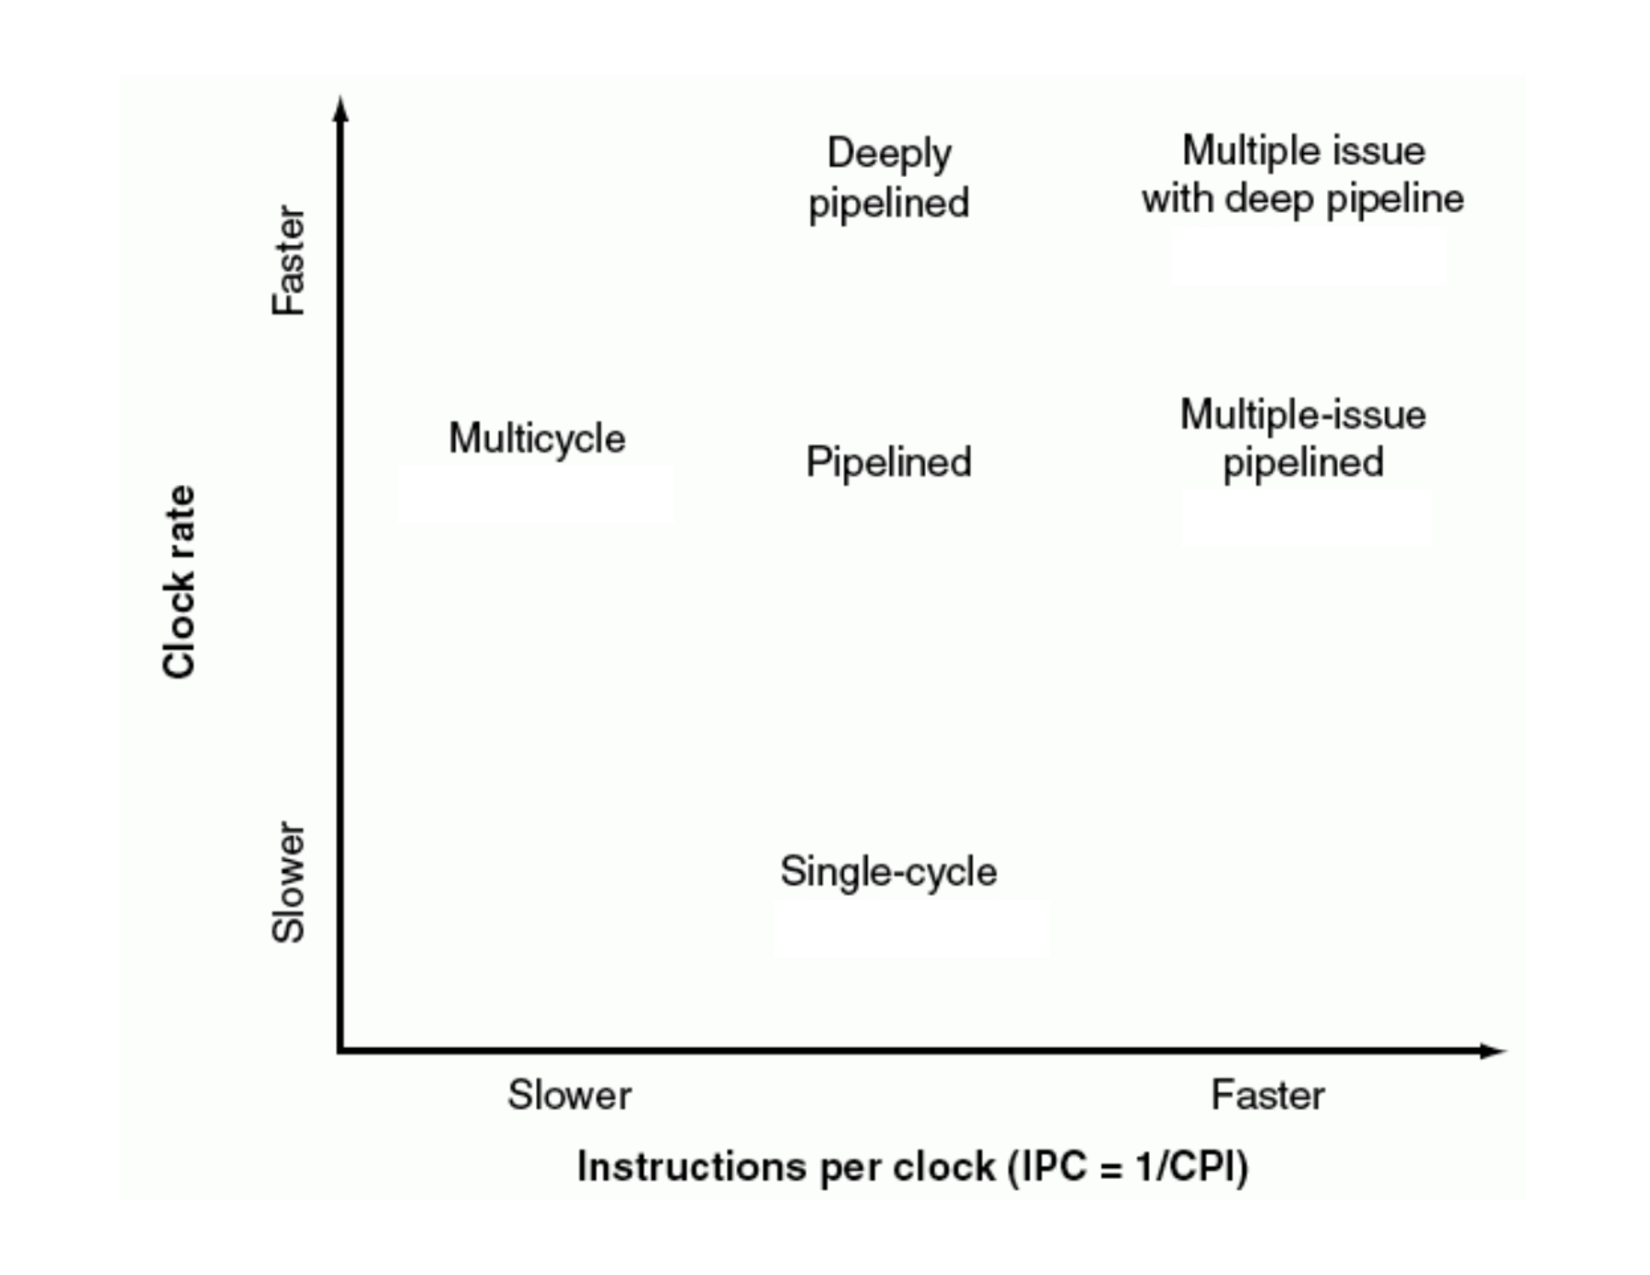
\includegraphics[width=6in]{./pics/frequency-vs-ipc}
\caption{Plot of clock frequency versus instructions per clock cycle (IPC) \cite{Patterson2005}. $IPC = \frac{1}{CPI}$ (see Equation \ref{eqn:ipcandcpi}), where {\it CPI} refers to clock cycles per instruction (see Section \ref{sec:IntroProcessorArchitecture}). From the ``iron law'' in Equation \ref{eqn:ironlaw}, the clock rate (CCT) and IPC (or $\frac{1}{CPI}$) affects the performance of the processor. Hence, as we move from design solutions in the bottom-left corner towards those in the top-right corner, we can find design solutions that have better computer performance.}
\label{fig:frequencyvsipc}
\end{figure}

%In Figure \ref{fig:frequencyvsipc}, a plot of clock frequency (i.e., clock rate) versus instructions per clock cycle (IPC) is shown \cite[Figure 6.52, pp. 453]{Patterson2005}. {\it IPC} is determined as follows \cite{Shen2005a}:
In Figure \ref{fig:frequencyvsipc}, a plot of clock frequency (i.e., clock rate) versus instructions per clock cycle (IPC) is shown \cite{Patterson2005}. {\it IPC} is determined as follows \cite{Shen2005a}:
\begin{equation}
\label{eqn:ipcandcpi}
IPC = \frac{1}{CPI},
\end{equation}

where {\it CPI} refers to clock cycles per instruction (see Equation \ref{eqn:ironlaw}). The performance of a processor architecture design improves as design choices are enumerated from the bottom-left corner of Figure \ref{fig:frequencyvsipc} towards its top-right corner. Data and control dependences of instructions in any given computer program limit how much instruction-level parallelism (ILP) can be exploited with pipelining and multiple instruction issue (i.e., superscalar processor design) for out-of-order execution. Therefore, in modern superscalar processor designs, instruction scheduling, dynamic branch prediction, and hardware speculation are used to improve processor performance \cite{Patterson2005,Shen2005a,Hennessy2012}. \\

A plot of the amount of hardware resource sharing versus instruction latency is shown in Figure \ref{fig:amountofhwsharingvsinstructionlatency}. Like in Figure \ref{fig:frequencyvsipc}, the performance of a processor architecture design improves as design choices are enumerated from the bottom-left corner towards the top-right corner. As aforementioned, pipelining and the width of instruction issue cannot be increased indefinitely without incurring performance penalty; this is the ``ILP wall''. Recent history indicates that the ``memory wall'' and the ``power wall'' have become bottlenecks in microarchitecture design; the ``memory wall'' refers to the diverging rates of performance improvement between the processor and physical memory (i.e., main memory), and the ``power wall'' refers to the increasing power consumption of advanced processor designs from the late 1980s till the early 2000s. Hence, the processor design industry has shifted towards designing chip multiprocessors to improve computer performance \cite{Hennessy2012,Wulf1995}. \\

\begin{figure}[h]
\centering 
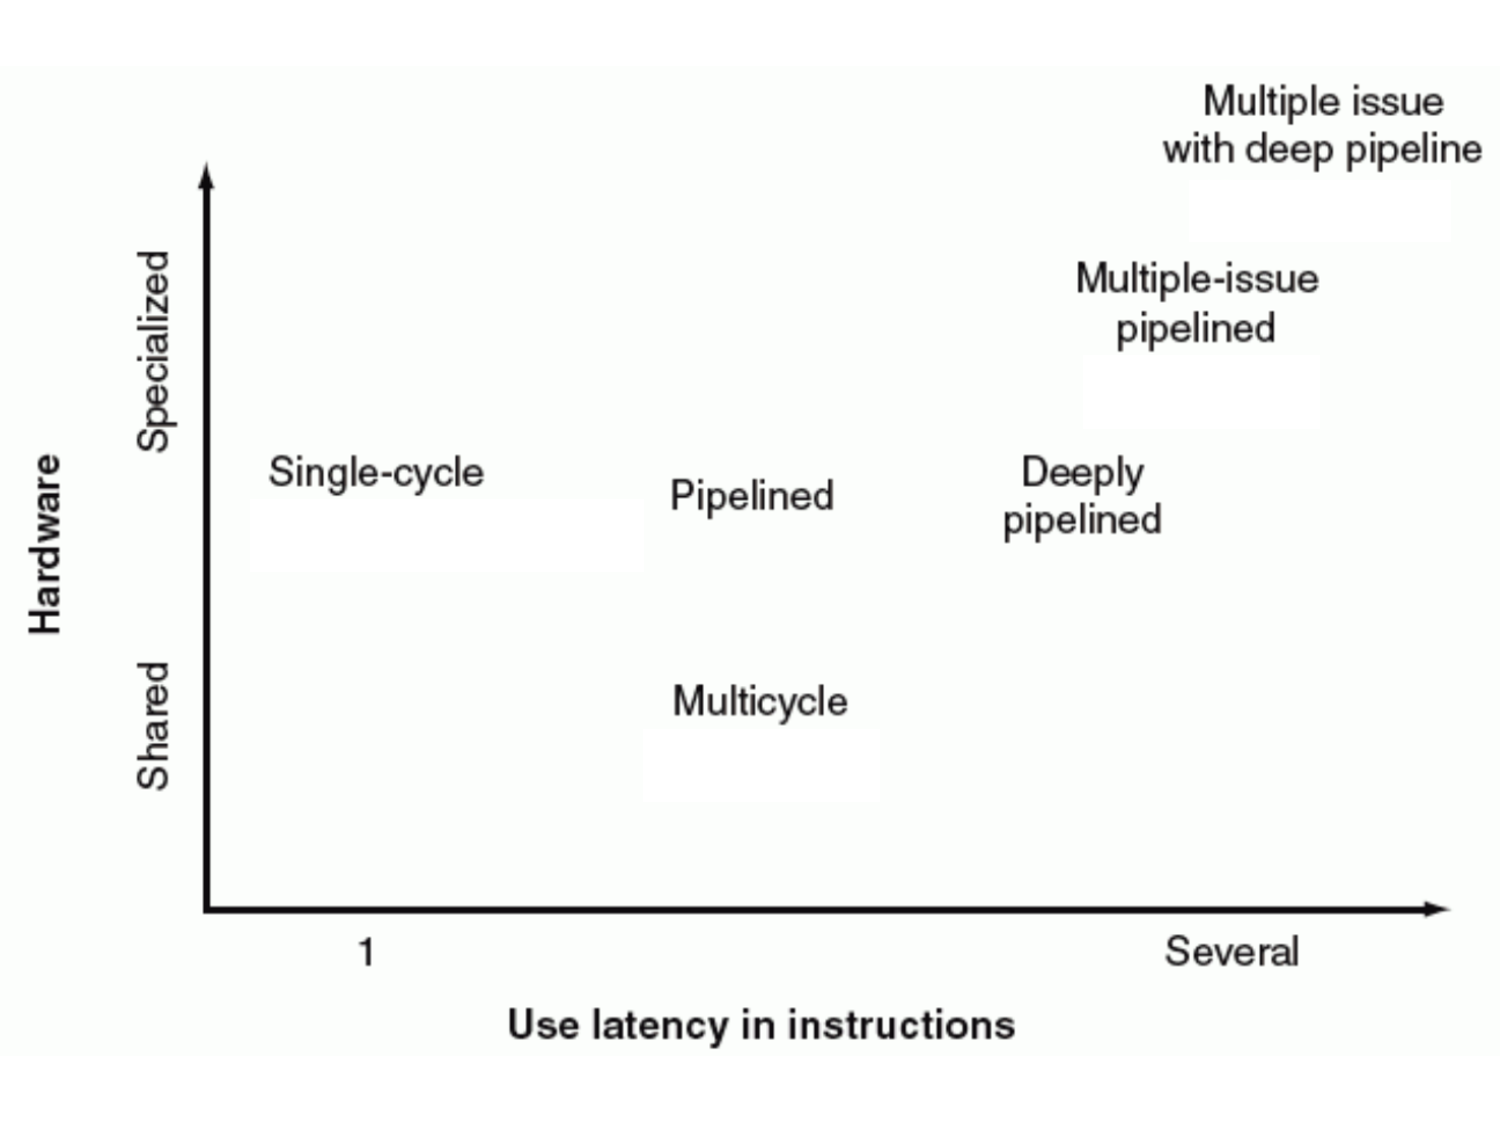
\includegraphics[width=6in]{./pics/amount-of-hw-sharing-vs-instruction-latency}
\caption{Plot of the amount of hardware resource sharing versus use latency in instructions \cite{Patterson2005}. The $y$-axis indicates the amount of specialized hardware that is used to execute instructions in a computer program, while the $x$-axis represents how easy it is to utilize all pipeline stages in a pipelined processor. As we move from design solutions in the bottom-left corner towards those in the top-right corner, we can find design solutions that have better computer performance.}
\label{fig:amountofhwsharingvsinstructionlatency}
\end{figure}



Hence, wisdom and insight about the applications that a processor would run can be used while considering trade-offs between hardware complexity (as well as design effort and power consumption) with performance. However, performance speedup need not come with only microarchitectural improvements. Performance speedup can also come from designing computer architectures for other computing paradigms (such as re-revisiting dataflow processor architectures \cite{Dennis1974}). It can also come using alternative computer system design paradigms, such as application-specific instruction set processors \cite{Gries2005,Karuri2011,Schliebusch2007}, neuromorphic processors \cite{Benjamin2014,Misra2010,Merolla2011,Seo2011,Kim2014,Kim2013a} and other cognitive computers, and general-purpose graphics processing units \cite{Altman2011,Kim2012,Kirk2010}. \\

Lastly, to paraphrase Prof. Roberto Sebastiani \cite{Sebastiani2007a}, neither the problem of designing an efficient processor architecture, nor that of acquiring a comprehensive background of microarchitecture is easy. The challenge of designing high-performance, energy-efficient processor architectures is not just a daunting engineering task, but also an art in itself.























